\subsection{Chapter 1 - The Scientific Method and Physics}

\subsubsection{Overview}\label{chap:introduction}

\begin{framed}
\textbf{Learning Objectives}\\
\begin{itemize}
\item Understand the Scientific Method.
\item Define the scope of Physics.
\item Understand the difference between theory and model.
\item Have a sense of how a physicist thinks.
\end{itemize}
\end{framed}

\begin{framed}
\textbf{Think About It}\\
A scientific theory...

\begin{enumerate}
\item must explain the physical world, and it may or may not be experimentally verifiable.
\item proves our models to be correct, and it must be experimentally verifiable.
\item describes the physical world, and must be experimentally verifiable.
\item must disprove other theories, and may or may not be experimentally verifiable.
\end{enumerate}

\begin{framed}
\textbf{Answer}\\
\begin{enumerate}[resume]
\item
\end{enumerate}
\end{framed}
\end{framed}

\subsubsection{Science and the Scientific Method}

Science is the process of \textit{describing} the world around us. It is important to note that describing the world around us is not the same as \textit{explaining} the world around us. Science aims to answer the question ``How?'' and not the question ``Why?''. As we develop our description of the physical world, you should remember this important distinction and resist the urge to ask ``Why?''.

The Scientific Method is a prescription for coming up with a description of the physical world that anyone can challenge and improve through performing experiments. If we come up with a description that can describe many observations, or the outcome of many different experiments, then we usually call that description a ``Scientific Theory''. We can get some insight into the Scientific Method through a simple example.

Imagine that we wish to describe how long it takes for a tennis ball to reach the ground after being released from a certain height. One way to proceed is to describe how long it takes for a tennis ball to drop $1 {\rm m}$, and then to describe how long it takes for a tennis ball to drop $2 {\rm m}$, etc. We could generate a giant table showing how long it takes a tennis ball to drop from any given height. Someone would then be able to perform an experiment to measure how long a tennis ball takes to drop from $1 {\rm m}$ or $2 {\rm m}$ and see if their measurement disagrees with the tabulated values. If we collected the descriptions for all possible heights, then we would effectively have a valid and testable scientific theory that describes how long it takes tennis balls to drop from any height.

Suppose that a budding scientist, let's call her Chloe, then came along and noticed that there is a pattern in the theory that can be described much more succinctly and generally than by using a giant table. In particular, suppose that she notices that, mathematically, the time, $t$, that it takes for a tennis ball to drop a height, $h$, is proportional to the square root of the height:
\begin{equation}
t \propto \sqrt{h}
\end{equation}

\begin{framed}
\textbf{Example}\\
Use Chloe's Theory ($t \propto \sqrt{h}$) to determine how much longer it will take for an object to drop by $2 {\rm m}$ than it would to drop by $1 {\rm m}$.

\begin{framed}
\textbf{Solution}\\
When we have a proportionality law (with a $\propto$) sign, we can always change this to an equal sign by introducing a constant, which we will call $k$:
\begin{equation}
t &\propto \sqrt{h} \\
\rightarrow t&=k\sqrt{h}
\end{equation}
Let $t_1$ be the time to fall a distance $h_1=1 {\rm m}$, and $t_2$ be the time to fall a distance $h_2=2 {\rm m}$. In terms of our unknown constant, $k$, we have:
\begin{equation}
t_1 &=k\sqrt{h_1}=k \sqrt{(1 {\rm m})}\\
t_2 &=k\sqrt{h_2}=k \sqrt{(2 {\rm m})}\\
\end{equation}
By taking the ratio, $\frac{t_1}{t_2}$, our unknown constant $k$ will cancel:
\begin{equation}
\frac{t_1}{t_2}&=\frac{\sqrt{(1 {\rm m})}}{\sqrt{(2 {\rm m})}}=\frac{1}{\sqrt 2}\\
\therefore t_2 &= \sqrt{2} t_1
\end{equation}
and we find that it will take $\sqrt{2}\sim 1.41$ times longer to drop by $2 {\rm m}$ than it will by $1 {\rm m}$.
\end{framed}
\end{framed}

Chloe's ``Theory of Tennis Ball Drop Times'' is appealing because it is succinct, and it also allows us to make \textbf{verifiable predictions}. That is, using this theory, we can predict that it will take a tennis ball $\sqrt 2$ times longer to drop from $2 {\rm m}$ than it will from $1 {\rm m}$, and then perform an experiment to verify that prediction. If the experiment agrees with the prediction, then we conclude that Chloe's theory adequately describes the result of that particular experiment. If the experiment does not agree with the prediction, then we conclude that the theory is not an adequate description of that experiment, and we try to find a new theory.

Chloe's theory is also appealing because it can describe not only tennis balls, but the time it takes for other objects to fall as well. Scientists can then set out to continue testing her theory with a wide range of objects and drop heights to see if it describes those experiments as well. Inevitably, they will discover situations where Chloe's theory fails to adequately describe the time that it takes for objects to fall (can you think of an example?).

We would then develop a new ``Theory of Falling Objects'' that would include Chloe's theory that describes most objects falling, and additionally, a set of descriptions for the fall times for cases that are not described by Chloe's theory. Ideally, we would seek a new theory that would also describe the new phenomena not described by Chloe's theory in a succinct manner. There is of course no guarantee, ever, that such a theory would exist; it is just an optimistic hope of physicists to find the most general and succinct description of the physical world. This is a general difference between physics and many of the other sciences. In physics, one always tries to arrive at a succinct theory (e.g. an equation) that can describe many phenomena, whereas the other sciences are often very descriptive. For example, there is no succinct formula for how butterflies look; rather, there is a giant collection of observations of different butterflies.

This example highlights that applying the Scientific Method is an iterative process. Loosely, the prescription for applying the Scientific Method is:

\begin{enumerate}
\item Identify and describe a process that is not currently described by a theory.
\item Look at similar processes to see if they can be described in a similar way.
\item Improve the description to arrive at a ``Theory'' that can be generalized to make predictions.
\item Test predictions of the theory on new processes until a prediction fails.
\item Improve the theory.
\end{enumerate}

\begin{framed}
\textbf{Checkpoint}\\
Fill in the blanks: Physics is a branch of science that \_\_\_\_\_\_\_\_\_\_\_ the behaviour of the universe. When doing physics, we attempt to answer the question of \_\_\_\_\_\_\_\_\_\_\_ things work the way they do.

\begin{enumerate}
\item explains
\item describes
\item how
\item why
\end{enumerate}

\begin{framed}
\textbf{Answer}\\
\begin{enumerate}
\item describes
\item how
\end{enumerate}
\end{framed}
\end{framed}

\subsubsection{Theories, hypotheses and models}

For the purpose of this textbook (and science in general), we introduce a distinction in what we mean by ``theory'', ``hypothesis'', and by ``model''. We will consider a ``theory'' to be a set of statements (or an equation) that gives us a broad description, applicable to several phenomena and that allows us to make verifiable predictions. For example, Chloe's Theory ($t \propto \sqrt{h}$) can be considered a theory. Specifically, we do not use the word theory in the context of ``I have a theory about this...''

A ``hypothesis'' is a consequence of the theory that one can test. From Chloe's Theory, we have the hypothesis that an object will take $\sqrt{2}$ times longer to fall from $1 {\rm m}$ than from $2 {\rm m}$. We can formulate the hypothesis based on the theory and then test that hypothesis. If the hypothesis is found to be invalidated by experiment, then either the theory is incorrect, or the hypothesis is not consistent with the theory.

A ``model'' is a situation-specific description of a phenomenon \textit{based on a theory}, that allows us to make a specific prediction. Using the example from the previous section, our theory would be that the fall time of an object is proportional to the square root of the drop height, and a model would be applying that theory to describe a tennis ball falling by $4.2 {\rm m}$. From the model, we can form a testable hypothesis of how long it will take the tennis ball to fall that distance. It is important to note that a model will almost always be an approximation of the theory applied to describe a particular phenomenon. For example, if Chloe's Theory is only valid in vacuum, and we use it to model the time that it takes for an object to fall at the surface of the Earth, we may find that our model disagrees with experiment. We would not necessarily conclude that the theory is invalidated, if our model did not adequately apply the theory to describe the phenomenon (e.g. by forgetting to include the effect of air drag).

This textbook will introduce the theories from Classical Physics, which were mostly established and tested between the seventeenth and nineteenth centuries. We will take it as given that readers of this textbook are not likely to perform experiments that challenge those well-established theories. The main challenge will be, given a theory, to define a model that describes a particular situation, and then to test that model. This introductory physics course is thus focused on thinking of ``doing physics'' as the task of correctly modelling a situation.

\begin{framed}
\textbf{Emma's Thoughts}\\
\textbf{What's the difference between a model and a theory?}
``Model'' and ``Theory'' are sometimes used interchangeably among scientists. In physics, it is particularly important to distinguish between these two terms. A model provides an immediate understanding of something based on a theory.

For example, if you would like to model the launch of your toy rocket into space, you might run a computer simulation of the launch based on various theories of propulsion that you have learned. In this case, the model is the computer simulation, which describes what will happen to the rocket. This model depends on various theories that have been extensively tested such as Newton's Laws of motion, Fluid dynamics, etc.

\begin{itemize}
\item ``Model'': Your homemade rocket computer simulation
\item ``Theory'': Newton's Laws of motion, Fluid dynamics
\end{itemize}

With this analogy, we can quickly see that the ``model'' and ``theory'' are not interchangeable. If they were, we would be saying that all of Newton's Laws of Motion depend on the success of your piddly toy rocket computer simulation!
\end{framed}

\begin{framed}
\textbf{Checkpoint}\\
Models cannot be scientifically tested, only theories can be tested.\}

\begin{enumerate}
\item True
\item False
\end{enumerate}

\begin{framed}
\textbf{Answer}\\
\begin{enumerate}[resume]
\item
\end{enumerate}
\end{framed}
\end{framed}

\subsubsection{Fighting intuition}

It is important to remember to fight one's intuition when applying the scientific method. Certain theories, such as Quantum Mechanics, are very counter-intuitive. For example, in Quantum Mechanics, an object can be described as being in two locations at the same time. In the Theory of Special Relativity, it is possible for two people to disagree on whether two events occurred at the same time. These particular predictions from these theories have not been invalidated by any experiment.

There is no requirement in science that a theory be ``pretty'' or intuitive. The only requirement is that a theory describe experimental data. One should then take care in not forcing one's preconceived notions into interpreting a theory. For example, Quantum Mechanics does not actually predict that objects can be in two locations at once, only that objects behave \textit{as if} they were in two locations at once. A famous example is Schr"odinger's cat, which can be modelled as being both alive and dead at the same time. However, just because we model it that way does not mean that it really is alive and dead at the same time.

\subsubsection{The scope of Physics}

Physics describes a wide range of phenomena within the physical sciences, ranging from the behaviour of microscopic particles that make up matter to the evolution of the entire Universe. We often distinguish between ``classical'' and ``modern'' physics depending on when the theories were developed, and we can further subdivide these areas of physics depending on the scale or the type of the phenomena that they describe.

The word physics comes from Ancient Greek and translates to ``nature'' or ``knowledge of nature''. The goal of physics is to develop theories from which mathematical models can be derived to describe our observations. One of the ambitious goals of physicists is to develop a single theory that describes all of nature, instead of having multiple theories to describe different categories of phenomena. This is in stark contrast to other fields of science, as Rutherford famously quipped: ``All science is either physics or stamp collecting''. That is, physicists hope that there exists one single mathematical theory (like Chloe's theory of falling objects) that describes the entire physical world. In Biology, for example, this would not be a reasonable goal, as one needs to describe every single living being, and there is no overarching ``theory of what all living things look like''. Currently, physicists have been able to narrow down the number of theories required to describe all of the physical world to only three, which is impressive (the theory of gravity, the theory of the strong nuclear force, and physicists have now further unified the weak nuclear force with electromagnetism to make the ``electroweak force'').

\paragraph{Classical Physics}

This textbook is focused on classical physics, which corresponds to the theories that were developed before 1905.
{\textbackslash}subsubsection\{Mechanics\}
Mechanics describes most of our everyday experiences, such as how objects move, including how planets move under the influence of gravity. Isaac Newton was the first to formally develop a theory of mechanics, using his ``Three Laws'' to describe the behaviour of objects in our everyday experience. His famous work published in 1687, ``Philosophiae Naturalis Principia Mathematica'' (``The Principia'') also included a theory of gravity that describes the motion of celestial objects.

Following the 1781 discovery of the planet Uranus by William Herschel, astronomers noticed that the orbit of the planet was not well described by Newton's theory. This led Urbain Le Verrier (in Paris) and John Couch Adams (in Cambridge) to predict the location of a new planet that was disturbing the orbit of Uranus rather than to claim that Newton's theory was incorrect. The planet Neptune was subsequently discovered by Le Verrier in 1846, one year after the prediction, and seen as a resounding confirmation of Newton's theory.

In 1859, Urbain Le Verrier also noted that Mercury's orbit around the Sun is different than that predicted by Newton's theory. Again, a new planet was proposed, ``Vulcan'', but that planet was never discovered and the deviation of Mercury's orbit from Newton's prediction remained unexplained until 1915, when Albert Einstein introduced a new, more complete, theory of gravity, called ``General Relativity''. This is a good example of the scientific method; although the discovery of Neptune was consistent with Newton's theory, it did not prove that the theory is correct, only that it correctly described the motion of Uranus. The discrepancy that arose when looking at Mercury ultimately showed that Newtons' theory of gravity fails to provide a proper description of planetary orbits in the proximity of very massive objects (Mercury is the closest planet to the Sun).

\begin{framed}
\textbf{Checkpoint}\\
What did the inability to find the planet Vulcan show:\}

\begin{enumerate}
\item It showed that Newton's model of Mercury was correct.
\item It showed that Newton's theory did not correctly describe the orbits of all planets.
\item It showed that the technology at the time was inadequate.
\item It showed that Einstein's theory of General Relativity was correct.
\end{enumerate}

\begin{framed}
\textbf{Answer}\\
\begin{enumerate}[resume]
\item
\end{enumerate}
\end{framed}
\end{framed}

\paragraph{Electromagnetism}

Electromagnetism describes electric charges and magnetism. At first, it was not realized that electricity and magnetism were connected. Charles Augustin de Coulomb published in 1784 the first description of how electric charges attract and repel each other. Magnetism was discovered in the ancient world, when people noticed that lodestone (rocks made from magnetized magnetite mineral) could attract iron tools. In 1819, Oersted discovered that moving electric charges could influence a compass needle, and several subsequent experiments were carried out to discover how magnets and moving electric charges interact.

In 1865, James Clerk Maxwell published ``A Dynamical Theory of the Electromagnetic Field'', wherein he first proposed a theory that unified electricity and magnetism as two facets of the same phenomenon. One important concept from Maxwell's theory is that light is an electromagnetic wave with a well-defined speed. This uncovered some potential issues with the theory as it required an absolute frame of reference in which to describe the propagation of light. Experiments in the late 1800s failed to detect the existence of this frame of reference.

\paragraph{Modern Physics}

In 1905, Albert Einstein published three major papers that set the foundation for what we now call ``Modern Physics''. These papers covered the following areas that were not well-described by classical physics:

\begin{itemize}
\item A description of Brownian motion that implied that all matter is made of atoms.
\item A description of the photoelectric effect that implied that light is made of particles.
\item A description of the motion of very fast objects that implied that mass is equivalent to energy, and that time and distance are relative concepts.
\end{itemize}

In order to accommodate Einstein's descriptions, physicists had to dramatically re-formulate new theories.

\subparagraph{Quantum mechanics and particle physics}

Quantum mechanics is a theory that was developed in the 1920s to incorporate Einstein's conclusion that light is made of particles (or rather, quantized lumps of energy called quanta) and describe nature at the smallest scales. This could only be done at the expense of determinism, the idea that we can predict how particular situations evolve in time. This led to a theory that could only provide the \textit{probabilities} that certain outcomes will be realized. Quantum mechanics was further refined during the twentieth century into Quantum Field Theory, which led to the Standard Model of particle physics that describes our current understanding of matter through the theories of the electroweak and strong forces.

\subparagraph{The Special and General Theories of Relativity}

In 1905, Einstein published his ``Special Theory of Relativity'', which describes how light propagates at a constant speed without the need for an absolute frame of reference, thus solving the problem introduced by Maxwell. This required physicists to consider space and time on an equal footing (``space-time''), rather than two independent aspects of the natural world, and led to a flurry of odd, but verified, experimental predictions. One such prediction is that time flows slower for objects that are moving fast, which has been experimentally verified by flying precise atomic clocks on airplanes and satellites. In 1915, Einstein further refined his theory into General Relativity, which is our best current description of gravity and includes a description of Mercury's orbit which was not described by Newton's theory.

\begin{framed}
\textbf{Checkpoint}\\
Special relativity can be applied to which of these science fiction plots?

\begin{enumerate}
\item An eccentric duo travel back in time to alter the past.
\item An astronaut travelling near light speed for many years comes home to find that he has aged less than his family on Earth.
\item A superhero harnesses lightning to use as a weapon.
\end{enumerate}

\begin{framed}
\textbf{Answer}\\
\begin{enumerate}[resume]
\item
\end{enumerate}
\end{framed}
\end{framed}

\subparagraph{Cosmology and astrophysics}

Cosmology describes processes at the largest scales and is mostly based on applying General Relativity to the scale of the Universe. For example, cosmology describes how our Universe started from the Big Bang and how large scale structures, such as galaxies and clusters of galaxies, have formed and evolved into our present day Universe.

\begin{figure}[!htbp]
\centering
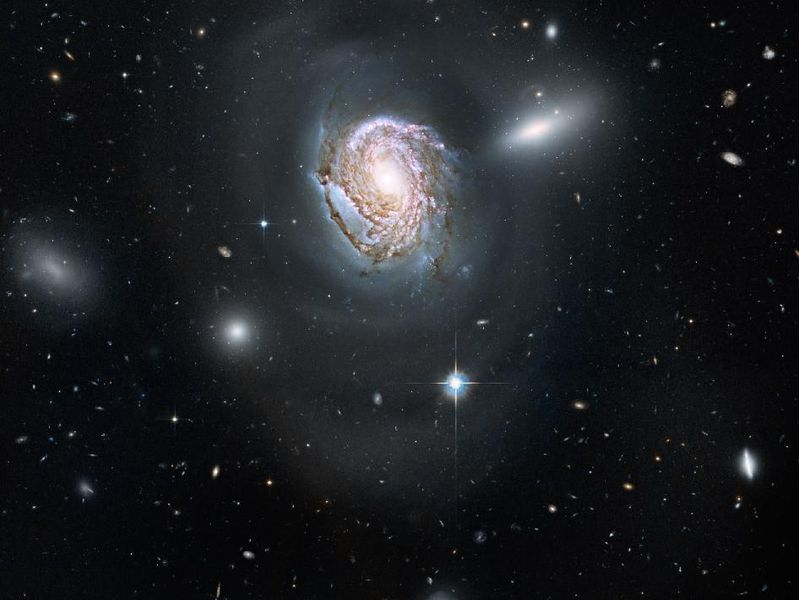
\includegraphics[width=0.6\linewidth]{files/galaxies_in_Coma_clu-2efab0f27a437395c54cadf99cecdeb8.jpeg}
\caption[]{A galaxy in the Coma cluster of galaxies (credit:NASA).}
\label{fig:introduction:galaxiescomacluster}
\end{figure}

Astrophysics is focused on describing the formation and the evolution of stars, galaxies, and other ``astrophysical objects'' such as neutron stars and black holes.

\subparagraph{Particle astrophysics}

Particle astrophysics is a relatively new field that makes use of subatomic particles produced by astrophysical objects to learn both about the objects \textit{and} about the particles. For example, the 2015 Nobel Prize in Physics was awarded to Art McDonald (a Canadian physicist from Queen's University) for using neutrinos\footnote{Neutrinos are the lightest subatomic particles that we know of.} produced by the Sun to both learn about the nature of neutrinos and about how the Sun works.

\subsubsection{Thinking like a physicist}

In a sense, physics can be thought of as the most fundamental of the sciences, as it describes the interactions of the smallest constituents of matter. In principle, if one can precisely describe how protons, neutrons, and electrons interact, then one can completely describe how a human brain thinks. In practice, the theories of particle physics lead to equations that are too difficult to solve for systems that include as many particles as a human brain. In fact, they are too difficult to solve exactly for even rather small systems of particles such as atoms bigger than helium (containing several protons, neutrons and electrons).

We have a number of other fields of science to cover complex systems of particles interacting. Chemistry can be used to describe what happens to systems consisting of many atoms and molecules. In a living being, it is too difficult to keep track of systems of atoms and molecules, so we use Biology to describe living systems.

One of the key qualities required to be an effective physicist is an ability to understand how to apply a theory and develop a model to describe a phenomenon. Just like any other skill, it takes practice to become good at developing models. Students that graduate with a physics degree are thus often sought for jobs that require critical thinking and the ability to develop quantitative models, which covers many fields from outside of physics such as finance or Big Data. This textbook thus tries to emphasize practice with developing models, while also providing a strong background in the theories of classical physics.

\subsubsection{Summary}

Science attempts to \textit{describe} the physical world (it answers the question ``How?'', not ``Why?'').

The Scientific Method provides a prescription for arriving at theories that describe the physical world and that can be experimentally verified. The Scientific Method is necessarily an iterative process where theories are continuously updated as new experimental data are acquired. An experiment can only disprove a theory, not confirm it in any general sense.

Physics covers a wide scale of phenomena ranging from the Universe down to subatomic particles. Classical physics encompasses the theories developed before 1905, when Einstein introduced the need for Quantum Mechanics and the Theorie(s) of Relativity. One of the main goals of physics is to arrive at a single theory that describes all of our natural world. Currently, physicists require three theories to describe the natural world.

\subsubsection{Thinking about the Material}

\begin{framed}
\textbf{Reflect and research}\\
\begin{itemize}
\item What particle helps to give mass to all of the massive elementary particles?
\item Name that physicist! Who was the first to propose that the universe is expanding?
\item Before discovering the CMBR (Cosmic Microwave Background Radiation), scientists Arno Penzias and Robert Wilson were trying to detect radio waves with very sensitive antennae. The very first time they heard a consistent, low noise on their detectors they discovered that it was (mostly) not the CMBR. What was causing most of this noise?
\item Physicist Lene Hau first slowed a beam of light to $17 {\rm m/s}$ using a very cold, dilute gas of bosons. In 2001, she improved on this result further; at which speed was she able to slow a beam of light?
\item Think of two theories that you use in your every day life. (For example, when we wash our hands, we do so because of the germ theory of disease!)
\end{itemize}
\end{framed}

\subsubsection{Sample problems and solutions}

\paragraph{Problems}

\begin{framed}
\textbf{Problem 1.1}\\
Your friend Martin loves to explore ``conspiracy theories''. His favourite theory involves ``Chem Trails''. He tells you that the government is secretly using airliners to spread chemicals in the atmosphere for some unknown reason.

\begin{itemize}
\item Think of 2 ways in which you could objectively test Martin's theory.
\item After proposing your experiment to Martin, he claims that his theory cannot be invalidated by any experiment, no matter how scientifically rigorous the experiment is. Is Martin correct?
\end{itemize}
\end{framed}

\paragraph{Solutions}

\begin{framed}
\textbf{Solution .1}\\
\begin{itemize}
\item a) You could do an investigation to see if the government is spreading chemicals, and try to find out why. You could make measurements of the contents in the atmosphere before and after an airline passes to see if any unexpected chemicals show up.


\item b) No he is not, as you just proposed two experiments that could invalidate his theory.
\end{itemize}
\end{framed}